\documentclass[11pt,twoside]{hsrthesis}

\makeindex

% do this here, so you can \gls{...} to it
%add new glossaryentries here...

\newglossaryentry{sqlite}{
	name=SQLite,
	description={SQLite ist eine Datenbankengine, welche ohne Konfiguration auskommt. Es handelt sich dabei um eine Datenbank in einer Datei},
	first={SQLite}
}
\makeglossaries

\begin{document}

\newcommand{\thesistitle}{OSM Crosswalk Detection}
\newcommand{\thesisauthora}{Bühler Severin}
\newcommand{\thesisauthorb}{Kurath Samuel}
\newcommand{\thesisauthorc}{}
\newcommand{\professor}{Prof. Keller Stefan}
\newcommand{\thesistype}{Semesterarbeit}
\newcommand{\departement}{Abteilung Informatik}
\newcommand{\school}{Hochschule für Technik Rapperswil}
\newcommand{\term}{Herbstsemester 2015}
\newcommand{\thedate}{18. Dezember 2015}
\newcommand{\timeperiode}{16.09.2015 - 18.12.2015}
\newcommand{\workload}{240 Stunden, 8 ECTS pro Student}
\newcommand{\linktothesis}{https://github.com/geometalab/OSM-Crosswalk-Detection}

\setlength{\oddsidemargin}{20mm}
\maketitle
\setlength{\oddsidemargin}{20mm}


\tableofcontents


% The main content
%%%%%%%%%%%%%%%%%%
\chapter*{Abstract}

Zebrastreifen sind ein essentieller Bestandteil der Fussgängernavigation, diese sind jedoch nur spärlich erfasst, was zu nicht optimalen Routen führt. 
Um dem entgegen zu wirken,  befasst sich dieses Projekt mit der automatischen Erkennung von Zebrastreifen auf Orthofotos (Satellitenbildern). 
Dabei entstand eine Applikation, die auf den Orthofotos den Strassen folgt, diese in kleine Bilder unterteilt und mit Hilfe eines Deep learnig Ansatzes entscheidet, ob es sich um ein Zebrastreifen handelt oder nicht.
Das führte zu einer Erkennungsrate von über 85\% und könnte in Zukunft den Behöreden bei der Erfassung der Daten (derzeit noch händisch) unterstützen.
Weiter ist es möglich diese Lösung auszubauen und auf andere Objekte anzuwenden.

\chapter*{Management Summary}
\section{Ausgangslage}
Das Erfassen von Zebrastreifen geschieht heutzutage noch händisch durch die jeweiligen Behörden.
Dieses Projekt befasst sich damit, diesem noch manuel Vorgang einen automatisierten Aspekt zu verleihen.
Dabei wird auf Informationen zu Strassenverläufen und Orthofotos (Satellitenbilder) zurückgegriffen. 
\section{Ergebnisse}
Es soll eine Applikationen entstehen die mit dem Input von Strassen und Orthofotos Zebrastreifen erkennt und als Output die jeweiligen Koordinaten liefert.
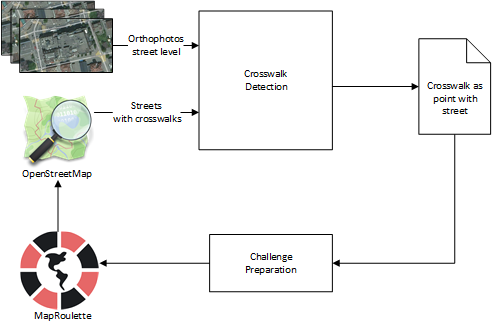
\includegraphics[width=\textwidth]{images/management_summary_1.png}
\section{Ausblick}
Das Projekt bietet viele Ausbaumöglichkeiten und kann nich nur auf Zebrastreifen angewendet werden. Es ist auch Denkbar auf den Strassen nach Markierungen zu suchen, wie Stop oder Bus etc.
\chapter{Technischer Bericht}
\chapter{Stand der Technik}
Um abzuklären, ob es schon Arbeiten gab, die ein ähnliches Problem lösen, nahmen wir uns im Rahmen der Semesterarbeit Zeit für ein Literaturrecherche. Dabei gingen wir auf die HSR Bibliothek und deren Mitarbeiter zu.
\section{Literaturrecherche}
\subsection{Suchquellen}
Folgende Quellen wurden uns empfohlen, um Recherchen in diesem Umfeld durchzuführen:
\begin{itemize}
	\item \url{http://recherche.nebis.ch/}
    \item \url{http://ieeexplore.ieee.org/}
    \item \url{http://scholar.google.ch/}
\end{itemize}

\subsection{Auswertung}
Bei der Recherche stiessen wir auf verschieden Projekte, die sich mit der Problematik des Erkennens von Fussgängerstreifen auseinander setzen. Leider sind diese Arbeiten eher im Bereich der Bilderkennung für die Steuerung von autonom fahrenden Autos/Robotern angesiedelt. Arbeiten die treffender sind, werden im Anschluss angeführt.
\subsection{Extraction of Road Markings from Aerial Images}
Yuichi Ishino und Hitoshi Saji (Japan, 2008) \newline 

\onehalfspacing 
\url{http://ieeexplore.ieee.org/stamp/stamp.jsp?tp=\&arnumber=4655024}
\onehalfspacing

An der Univerisität Shizuoka in Japan gab es vor einigen Jahren eine Arbeit zur Erkennung von Fussgängerstreifen und Mittellinien (Traffic Lane Lines) auf Orthofotos (Aerial images).

Ihr Algorithmus befolgt dabei folgende Strategie:
Der Algorithmus geht den Strassen entlang und richtet die Bilder aus, dass die Fussgängerstreifen immer vertikal zur Achse laufen. Danach wird eine sogenannte Binarization durchgeführt. Es setzt alle Pixel unter einem Schwellwert auf 0 (weiss) und alle Pixel darüber auf 1 (schwarz). Es wurden zwei Schwellwerte zurvor berechnet, einmal für sonnige und einmal für schattige Bilder.
Mit der Annahme, dass die Strasse schwarz/grau und der Fussgängerstreifen leuchtend weiss sind, sieht man nun ein gleichmässiges Muster in der Helligkeitsverteilung des Bildes. Ein Fouriertransformation würde eine saubere Frequenz liefern.

Die Arbeit von Ishino und Saji geht von einigen Grundannahmen und Vorraussetzungen aus, die die Erkennung sehr erleichtern:

\begin{itemize}
	\item Die Fussgängerstreifen sind immer gerade und werden durch keine Inseln unterbrochen.
	\item Die Auflösung der Bilder ist genug gross, um das Streifenmuster ohne Probleme zu erkennen.
	\item Der Fussgängerstreifen ist immer deutlich heller als die Strasse selbst.
	\item Der Streifen werden durch keine Hindernisse wie Bäume, Autos verdeckt oder beeinflusst.
	\item Die Bilder wurde zuvor in die Kategorien schattig und sonnig eingeteilt worden. Auf ihnen wird mit verschiedenen Treshholds gearbeitet.
	\item Die Strassen müssen die Fussgängerstreifen immer vertikal schneiden.
\end{itemize}

\subsubsection{Schlussfolgerung}
Die Arbeit der Univerisität von Shizuoka verfolgte einen ähnlichen Ansatz, den wir mit der Fouriertransformation in Betracht ziehen. Leider gehen die Dokumentverfasser von einigen Grundannahmen aus, die sich nicht mit der unseren Arbeit decken. Man kann fast schon von Laborbedingungen sprechen.
Doch gibt es einigen Techniken, die sich auch für unsere Arbeit verwenden lassen. Diese sind unten aufgeführt.

\subsection{Segmentation of Occluded Sidewalks in Satellite Images}
Turgay Senlet und Ahmed Elgammal, The State University of New Jersey, USA (2012) \newline

\onehalfspacing
\url{http://ieeexplore.ieee.org/stamp/stamp.jsp?tp=\&arnumber=6460256}
\onehalfspacing
\newline


Das Projekt von Turgay Selent und Ahmed Elgammal setzte sich mit der Erkennung von primär Gehwege (sidewalks) und Fussgängerstreifen auf Satellitenbildern auseinander.

Dabei waren die Hauptprobleme, dass viel Gehweg von Bäumen oder Schatten verdeckt werden. Um diesem Problem Herr zu werden, benutzten sie einen Farbklassifizierer.
Um Fussgängerstreifen zu klassifizieren stellten sie eine Sammlung an Frequenzen in allen möglichen Winkeln zusammen. 

Leider wird im Artikel zu dieser Arbeit nicht weiter in die Erkennungsmethoden eigegangen.

\section{Fazit}
Aus allen Arbeiten konnten wir doch einige Techniken finden, die uns die Erkennung erleichtern könnten. Diese sind hier aufgelistet:
\begin{itemize}
	\item Binarization image 
	\item Median Filter (für Verbesserung der Bildqualität von ungenauen Bildern)
\end{itemize}

\section{Evaluation Crowdsourcing-System}
\subsection{Kandidaten}
\begin{itemize}
	\item MapRoulette\footnote{\url{http://maproulette.org/}} 
	\item To-Fix\footnote{\url{http://osmlab.github.io/to-fix/\#/task/tigerdelta}}
\end{itemize}

\subsection{MapRoulette}
MapRoulette verwendet für ihre Challenges und Tasks ein einfaches JSON Format. Der erstellt werden Challenges mittels POST und mit PUT können diese upgedatet werden.

\subsection*{Beispiel Challenge}
\begin{tabbing}
    \hspace*{4cm}\=\hspace*{5cm}\= \kill
    Erstellen: \> POST /api/admin/challenge/<slug>  \\
    Updaten: \> PUT /api/admin/challenge/<slug> \\
    Challenge JSON: \\
\end{tabbing}		
\begin{python}
{
  "title": "Repair Motorways",
  "description": "Repair all motorways",
  "blurb": "The idea is to repair all motorways",
  "help": "Repair the ways where it is broken on the map",
  "instruction": "Look at the map for broken pieces.",
  "active": true,
  "difficulty": 2
}
\end{python}

\subsection*{Beispiel Task}
\begin{tabbing}
    \hspace*{4cm}\=\hspace*{5cm}\= \kill
    Erstellen: \> POST /api/admin/challenge/<slug>/task/<task\_identifier> \\
    Updaten: \> PUT /api/admin/challenge/<slug>/task/<task\_identifier> \\
    Challenge JSON: \\
\end{tabbing}
\begin{python}
{ 
  "instruction" : "This is a hard task!",
  "geometries" : {
    "type": "FeatureCollection",
    "features": [
      { "type": "Feature",
        "geometry": 
        { "type": "Point", 
          "coordinates":[-41.4710170873565,31.235521774136]
        },
        "properties": {"osmid": 12345}
      }
    ]
  }
}
\end{python}	

\subsection{To-Fix}
To-Fix verwendet für ihre Task ein CSV Format, welches direkt über das grafische Benutzerinterface publiziert werden kann.
\subsection*{Beispiel CSV}
\begin{python}
object_type,object_id,st_astext
way,51446110,POINT(-94.4176451 43.3273692)
way,187403368,POINT(32.9369086 2.1997495)
way,220866128,POINT(-68.5 49.647521)
way,223982938,POINT(18.4823301 59.6732909)
way,109819283,POINT(-83.1888421 40.0485764)
\end{python}


\subsection{Evaluationsmatrix}
Um die beiden Kandidaten zu vergleich haben wir eine Evaluationsmatrix erstellt, dabei haben wir diverse für uns relevante Kriterien erarbeiten und diesen jeweils auf einer Skala von 1 bis 10 gewichtet.
In einem zweiten Schritt haben wir den Kandidaten für die jeweiligen Kriterien Punkte vergeben.

\begin{figure}[ht]
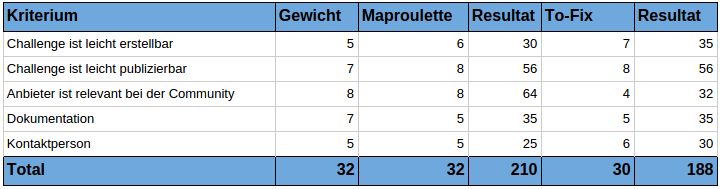
\includegraphics[width=\textwidth]{images/croud_evol_matrix.png}
\caption[Evaluationsmatrix]{Evaluationsmatrix}
\end{figure}

\decision{Crowdsourcing-System}
\decision{Crowdsourcing-System1}
\decision{Crowdsourcing-System2}
\subsubsection{Resultat}
Beide Kandidaten haben Vor- und Nachteile, wie aus der Evaluationsmatrix ersichtlich ist. Für uns ist das wichtigste Kriterium, wie relevant der Anbieter bei der Community ist, was sich dann auch im Resultat stark ausgewirkt hat. Da MapRoulette Challenges gerne abgearbeitet werden, tendieren wir für diesen Kandidaten.  

\chapter*{Examples}

\section*{Glossary Example}

\gls{sqlite} ist ein Glossar Eintrag. Lorem ipsum dolor sit amet, consetetur sadipscing elitr, sed diam nonumy eirmod tempor invidunt ut labore et dolore magna aliquyam erat, sed diam voluptua. At vero eos et accusam et justo duo dolores et ea rebum.

\section*{Bibliography and Citation Example}

Dies ist ein Zitat aus einem Buch\cite{Matthews201111}. Lorem ipsum dolor sit amet, consetetur sadipscing elitr, sed diam nonumy eirmod tempor invidunt ut labore et dolore magna aliquyam erat, sed diam voluptua. At vero eos et accusam et justo duo dolores et ea rebum.

Lorem ipsum dolor sit amet, consetetur sadipscing elitr, sed diam nonumy eirmod tempor invidunt ut labore et dolore magna aliquyam erat, sed diam voluptua. At vero eos et accusam et justo duo dolores et ea rebum. Stet clita kasd gubergren, no sea takimata sanctus est Lorem ipsum dolor sit amet. Lorem ipsum dolor sit amet, consetetur sadipscing elitr, sed diam nonumy eirmod tempor invidunt ut labore et dolore magna aliquyam erat, sed diam voluptua. At vero eos et accusam et justo duo dolores et ea rebum. Stet clita kasd gubergren, no sea takimata sanctus est Lorem ipsum dolor sit amet. Lorem ipsum dolor sit amet, consetetur sadipscing elitr, sed diam nonumy eirmod tempor invidunt ut labore et dolore magna aliquyam erat, sed diam voluptua. At vero eos et accusam et justo duo dolores et ea rebum. Stet clita kasd gubergren, no sea takimata sanctus est Lorem ipsum dolor sit amet. 

Duis autem vel eum iriure dolor in hendrerit in vulputate velit esse molestie consequat, vel illum dolore eu feugiat nulla facilisis at vero eros et accumsan et iusto odio dignissim qui blandit praesent luptatum zzril delenit augue duis dolore te feugait nulla facilisi. Lorem ipsum dolor sit amet, consectetuer adipiscing elit, sed diam nonummy nibh euismod tincidunt ut laoreet dolore magna aliquam erat volutpat. 

Ut wisi enim ad minim veniam, quis nostrud exerci tation ullamcorper suscipit lobortis nisl ut aliquip ex ea commodo consequat. Duis autem vel eum iriure dolor in hendrerit in vulputate velit esse molestie consequat, vel illum dolore eu feugiat nulla facilisis at vero eros et accumsan et iusto odio dignissim qui blandit praesent luptatum zzril delenit augue duis dolore te feugait nulla facilisi. 


\section*{Table Examples}
\subsection*{Automagical Column Widths}
\begin{tabularx}{\textwidth}{X X X X} \beforeheading
\heading{Heading 1} & \heading{Heading 2} & \heading{Heading 3} & \heading{Heading 4} \\\afterheading
Cell 1,1 & Cell 1,2 & Cell 1,3 & Cell 1,4 \\\normalline
Cell 2,1 & Cell 2,2 & Cell 2,3 Vel illum dolore eu feugiat nulla facilisis at vero eros et accumsan et iusto odio dignissim qui blandit praesent luptatum zzril delenit augue duis dolore te feugait nulla facilisi. & Cell 2,4 \\\normalline
Cell 3,1 Duis autem vel eum iriure dolor in hendrerit in vulputate velit esse molestie consequat. & Cell 3,2 & Cell 3,3 & Cell 3,4 \\\lastline
\end{tabularx}

\subsection*{Column Alignment \& Filler}
\begin{tabularx}{\textwidth}{l c r X} \beforeheading
\heading{Left Aligned} & \heading{Centered} & \heading{Right Aligned} & \heading{Filler} \\\afterheading
Cell 1,1 & Cell 1,2 & Cell 1,3 & Cell 1,4 Ut wisi enim ad minim veniam, quis nostrud exerci tation ullamcorper  \\\normalline
Cell 2,1 & Cell 2,2 & Cell 2,3 & Cell 2,4 Ut wisi enim ad minim veniam, quis nostrud exerci tation ullamcorper  \\\normalline
Cell 3,1 & Cell 3,2 & Cell 3,3 & Cell 3,4 Ut wisi enim ad minim veniam, quis nostrud exerci tation ullamcorper  \\\lastline
\end{tabularx}
%03introduction.tex

\chapter{Introduction}

In this thesis, the problem of solving something is being discussed. Lorem ipsum dolor sit amet, consectetur adipiscing elit. Sed gravida mollis placerat. Sed congue iaculis massa vitae dapibus. Fusce sed felis lorem. Suspendisse purus diam, sollicitudin vitae imperdiet ac, placerat eu metus. In luctus, metus vel dictum hendrerit, diam lacus cursus enim, eu porta augue lacus non metus. Pellentesque habitant morbi tristique senectus et netus et malesuada fames ac turpis egestas. Nullam nec orci eget metus pulvinar sagittis. Vestibulum ante ipsum primis in faucibus orci luctus et ultrices posuere cubilia Curae; Sed turpis lorem, aliquet eu ornare non, viverra ac urna.

Praesent libero lectus, ultrices eget pharetra sed, sollicitudin et est. Pellentesque quis urna eget lorem sodales venenatis eget nec quam. In sagittis aliquam auctor. Phasellus vitae ipsum purus, sit amet imperdiet nunc. Pellentesque habitant morbi tristique senectus et netus et malesuada fames ac turpis egestas. Ut malesuada nibh ut lectus scelerisque sed iaculis lectus varius. Nulla blandit turpis tortor. Nulla facilisi. Cum sociis natoque penatibus et magnis dis parturient montes, nascetur ridiculus mus. Nam leo ante, porta vel scelerisque at, volutpat eu sapien. Aliquam viverra adipiscing sapien et porta. Sed quis diam ut sem tincidunt consectetur varius non dolor. Fusce fermentum, quam vitae suscipit euismod, leo erat malesuada ante, ac consequat est lacus eget enim. Proin lacinia justo et est vehicula adipiscing rhoncus lacus mollis.

\section{Lorem}
Lorem ipsum dolor sit amet, consectetur adipiscing elit. Sed gravida mollis placerat. Sed congue iaculis massa vitae dapibus. Fusce sed felis lorem. Suspendisse purus diam, sollicitudin vitae imperdiet ac, placerat eu metus. In luctus, metus vel dictum hendrerit, diam lacus cursus enim, eu porta augue lacus non metus. Pellentesque habitant morbi tristique senectus et netus et malesuada fames ac turpis egestas. Nullam nec orci eget metus pulvinar sagittis. Vestibulum ante ipsum primis in faucibus orci luctus et ultrices posuere cubilia Curae; Sed turpis lorem, aliquet eu ornare non, viverra ac urna.

Praesent libero lectus, ultrices eget pharetra sed, sollicitudin et est. Pellentesque quis urna eget lorem sodales venenatis eget nec quam. In sagittis aliquam auctor. Phasellus vitae ipsum purus, sit amet imperdiet nunc. Pellentesque habitant morbi tristique senectus et netus et malesuada fames ac turpis egestas. Ut malesuada nibh ut lectus scelerisque sed iaculis lectus varius. Nulla blandit turpis tortor. Nulla facilisi. Cum sociis natoque penatibus et magnis dis parturient montes, nascetur ridiculus mus. Nam leo ante, porta vel scelerisque at, volutpat eu sapien. Aliquam viverra adipiscing sapien et porta. Sed quis diam ut sem tincidunt consectetur varius non dolor. Fusce fermentum, quam vitae suscipit euismod, leo erat malesuada ante, ac consequat est lacus eget enim. Proin lacinia justo et est vehicula adipiscing rhoncus lacus mollis.	

% \input{chapter/04mychapter}
% ...


% List of figures & glossary
%%%%%%%%%%%%%%%%%%%%%%%%%%%%
\listoffigures
\printglossary[style=altlist,title=Glossar]

% Bibliography
%%%%%%%%%%%%%%
\bibliographystyle {alpha}
\bibliography{index/bibliography}


% Attached sources
%%%%%%%%%%%%%%%%%%
 \input{attachments/attachments}


\end{document}